\subsection{M.PC.MS - Metriche Soddisfatte}

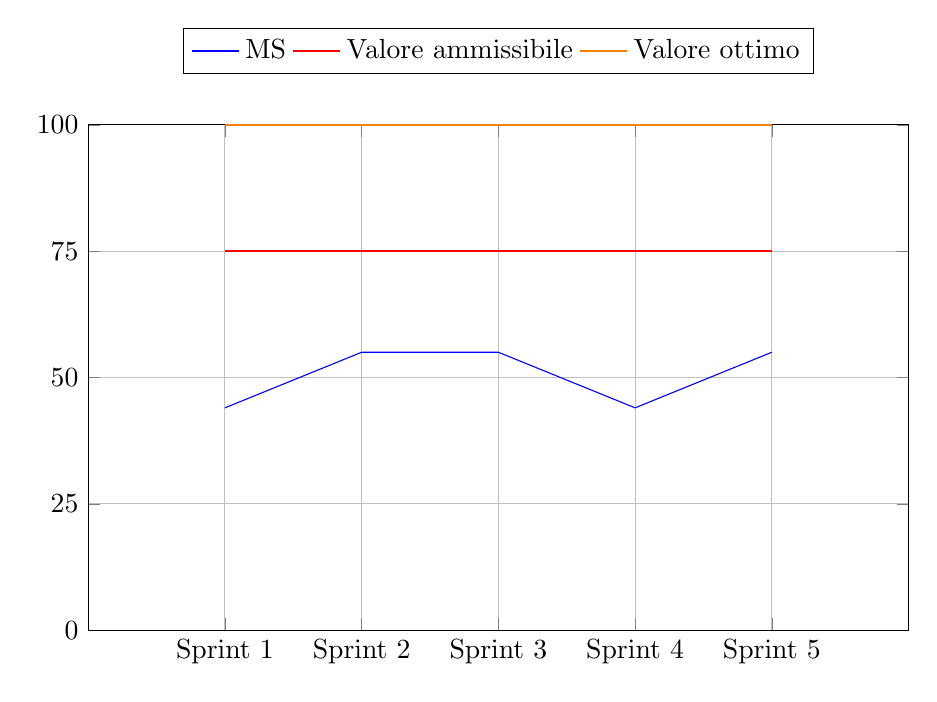
\begin{tikzpicture}
    \begin{axis}[
        width=12cm, height=8cm,
        ymin=0, ymax=100,
        xmin=0, xmax=6,
        ytick distance=25,
        xtick={1, 2, 3, 4, 5},
        xticklabels={Sprint 1, Sprint 2, Sprint 3, Sprint 4, Sprint 5},
        xlabel={},
        ylabel={},
        grid=major,
        scaled ticks=false,
        legend style={at={(0.5,1.1)}, anchor=south, legend columns=-1},
    ]
    \addplot[color=blue] coordinates {(1, 44) (2, 55) (3, 55) (4, 44) (5, 55)};
    \addlegendentry{MS}
    \addplot[red, thick] coordinates {(1, 75) (5, 75)};
    \addlegendentry{Valore ammissibile}
    \addplot[orange, thick] coordinates {(1, 100) (5, 100)};
    \addlegendentry{Valore ottimo}
    \end{axis}
\end{tikzpicture}
\subsubsection{RTB}
Non è stata assicurata la qualità che si voleva raggiungere per la realizzazione del progetto, i valori inferiori al valore ammissibile sono dovuti
dalle metriche di Schedule Variance, Cost Variance e Variazione del Piano che non hanno mai raggiunto il valore ammissibile durante lo svolgimento del progetto 
indicando una metodologia di lavoro che non è migliorata sufficientemente con il passare del tempo.